\documentclass{beamer}\usepackage[]{graphicx}\usepackage[]{color}
%% maxwidth is the original width if it is less than linewidth
%% otherwise use linewidth (to make sure the graphics do not exceed the margin)
\makeatletter
\def\maxwidth{ %
  \ifdim\Gin@nat@width>\linewidth
    \linewidth
  \else
    \Gin@nat@width
  \fi
}
\makeatother

\definecolor{fgcolor}{rgb}{0.196, 0.196, 0.196}
\newcommand{\hlnum}[1]{\textcolor[rgb]{0.063,0.58,0.627}{#1}}%
\newcommand{\hlstr}[1]{\textcolor[rgb]{0.063,0.58,0.627}{#1}}%
\newcommand{\hlcom}[1]{\textcolor[rgb]{0.588,0.588,0.588}{#1}}%
\newcommand{\hlopt}[1]{\textcolor[rgb]{0.196,0.196,0.196}{#1}}%
\newcommand{\hlstd}[1]{\textcolor[rgb]{0.196,0.196,0.196}{#1}}%
\newcommand{\hlkwa}[1]{\textcolor[rgb]{0.231,0.416,0.784}{#1}}%
\newcommand{\hlkwb}[1]{\textcolor[rgb]{0.627,0,0.314}{#1}}%
\newcommand{\hlkwc}[1]{\textcolor[rgb]{0,0.631,0.314}{#1}}%
\newcommand{\hlkwd}[1]{\textcolor[rgb]{0.78,0.227,0.412}{#1}}%
\let\hlipl\hlkwb

\usepackage{framed}
\makeatletter
\newenvironment{kframe}{%
 \def\at@end@of@kframe{}%
 \ifinner\ifhmode%
  \def\at@end@of@kframe{\end{minipage}}%
  \begin{minipage}{\columnwidth}%
 \fi\fi%
 \def\FrameCommand##1{\hskip\@totalleftmargin \hskip-\fboxsep
 \colorbox{shadecolor}{##1}\hskip-\fboxsep
     % There is no \\@totalrightmargin, so:
     \hskip-\linewidth \hskip-\@totalleftmargin \hskip\columnwidth}%
 \MakeFramed {\advance\hsize-\width
   \@totalleftmargin\z@ \linewidth\hsize
   \@setminipage}}%
 {\par\unskip\endMakeFramed%
 \at@end@of@kframe}
\makeatother

\definecolor{shadecolor}{rgb}{.97, .97, .97}
\definecolor{messagecolor}{rgb}{0, 0, 0}
\definecolor{warningcolor}{rgb}{1, 0, 1}
\definecolor{errorcolor}{rgb}{1, 0, 0}
\newenvironment{knitrout}{}{} % an empty environment to be redefined in TeX

\usepackage{alltt}

% load packages
\usepackage{tikz}
\usepackage{graphicx}
\usepackage{upquote}
\usepackage{listings}
\usepackage{hyperref}
\usepackage{color}
\usepackage{lmodern}

% define a bunch of colors
\definecolor{gray}{RGB}{110,110,110}
\definecolor{darkgray}{RGB}{100,100,100}
\definecolor{lightgray}{RGB}{200,200,200}
\definecolor{lightgrey}{RGB}{200,200,200}
\definecolor{turquoise}{RGB}{81,193,188}
\definecolor{mamey}{RGB}{255,107,107}
\definecolor{tomato}{RGB}{255,136,136}
\definecolor{mandarina}{RGB}{229,169,25}
\definecolor{lemon}{rgb}{0.81,0.95,0.29}
\definecolor{bluesky}{rgb}{0.71,0.81,0.96}
\definecolor{chiclamino}{RGB}{107,174,214}
\definecolor{violet}{RGB}{133,135,211}

\definecolor{foreground}{RGB}{81,141,193}
\definecolor{background}{RGB}{246,244,240}
\definecolor{highlight}{RGB}{229,169,25}
\definecolor{lowlight}{RGB}{200,200,200}

% setting beamer colors
\setbeamercolor{title}{fg=lightgray}
\setbeamercolor{frametitle}{fg=lightgray}
\setbeamercolor{block title}{fg=turquoise}
\setbeamercolor{structure}{fg=turquoise}
\setbeamercolor{titlelike}{fg=title}
\setbeamercolor{subtitle}{fg=turquoise}
\setbeamercolor{institute}{fg=gray}
\setbeamercolor{normal text}{fg=gray,bg=background}

\setbeamercolor{palette primary}{fg=lightgray}
\setbeamercolor{palette secondary}{fg=lightgray}
\setbeamercolor{palette tertiary}{fg=lightgray}

\setbeamerfont{itemize/enumerate subbody}{size=\footnotesize}
\setbeamerfont{itemize/enumerate subitem}{size=\footnotesize}

\hypersetup{
  colorlinks=true,
  urlcolor=tomato,
  linkcolor=lightgray
}

% commands
\newcommand{\code}[1]{\texttt{#1}}
\newcommand{\high}[1]{\textcolor{highlight}{#1}}
\newcommand{\low}[1]{\textcolor{lowlight}{#1}}
\newcommand{\highcode}[1]{\textcolor{highlight}{\texttt{#1}}}


%\usecolortheme{rose}
\setbeamertemplate{blocks}[rounded]
\setbeamertemplate{footline}[frame number] 
\setbeamertemplate{navigation symbols}{}
\setbeamertemplate{frametitle}[default][center]
\useoutertheme{infolines}  % add footlines
\setbeamersize{text margin left=25pt,text margin right=25pt}


\title[Getting data from the web with R]{\LARGE Getting Data from the Web with R} 
\subtitle[Web Data in R]{\large Part 7: Getting Data via Web Forms}
\author[gastonsanchez.com]{
 \textcolor{gray}{\textbf{G}aston \textbf{S}anchez}
}
\institute[]{\scriptsize \textcolor{lightgray}{April-May 2014}}
\date[CC BY-SA-NC 4.0]{
 \textcolor{lightgray}{\tiny{Content licensed under 
 \href{http://creativecommons.org/licenses/by-nc-sa/4.0/}{CC BY-NC-SA 4.0}}}
}

% to remove empty brackets of \institution
\makeatletter
\setbeamertemplate{footline}
{
  \leavevmode%
  \hbox{%
  \begin{beamercolorbox}[wd=.333333\paperwidth,ht=2.25ex,dp=1ex,center]{author in head/foot}%
    \usebeamerfont{author in head/foot}\insertshortauthor%~~\beamer@ifempty{\insertshortinstitute}{}{(\insertshortinstitute)}
  \end{beamercolorbox}%
  \begin{beamercolorbox}[wd=.333333\paperwidth,ht=2.25ex,dp=1ex,center]{title in head/foot}%
    \usebeamerfont{title in head/foot}\insertshorttitle
  \end{beamercolorbox}%
  \begin{beamercolorbox}[wd=.333333\paperwidth,ht=2.25ex,dp=1ex,right]{date in head/foot}%
    \usebeamerfont{date in head/foot}\insertshortdate{}\hspace*{2em}
    \insertframenumber{} / \inserttotalframenumber\hspace*{2ex} 
  \end{beamercolorbox}}%
  \vskip0pt%
}
\makeatother
\IfFileExists{upquote.sty}{\usepackage{upquote}}{}
\begin{document}



%--- the titlepage frame -------------------------%

\begin{frame}[plain]
 \titlepage
\end{frame}

%------------------------------------------------

{ % all template changes are local to this group.
    \setbeamertemplate{navigation symbols}{}
    \begin{frame}[plain]
        \begin{tikzpicture}[remember picture,overlay]
            \node[at=(current page.center)] {
                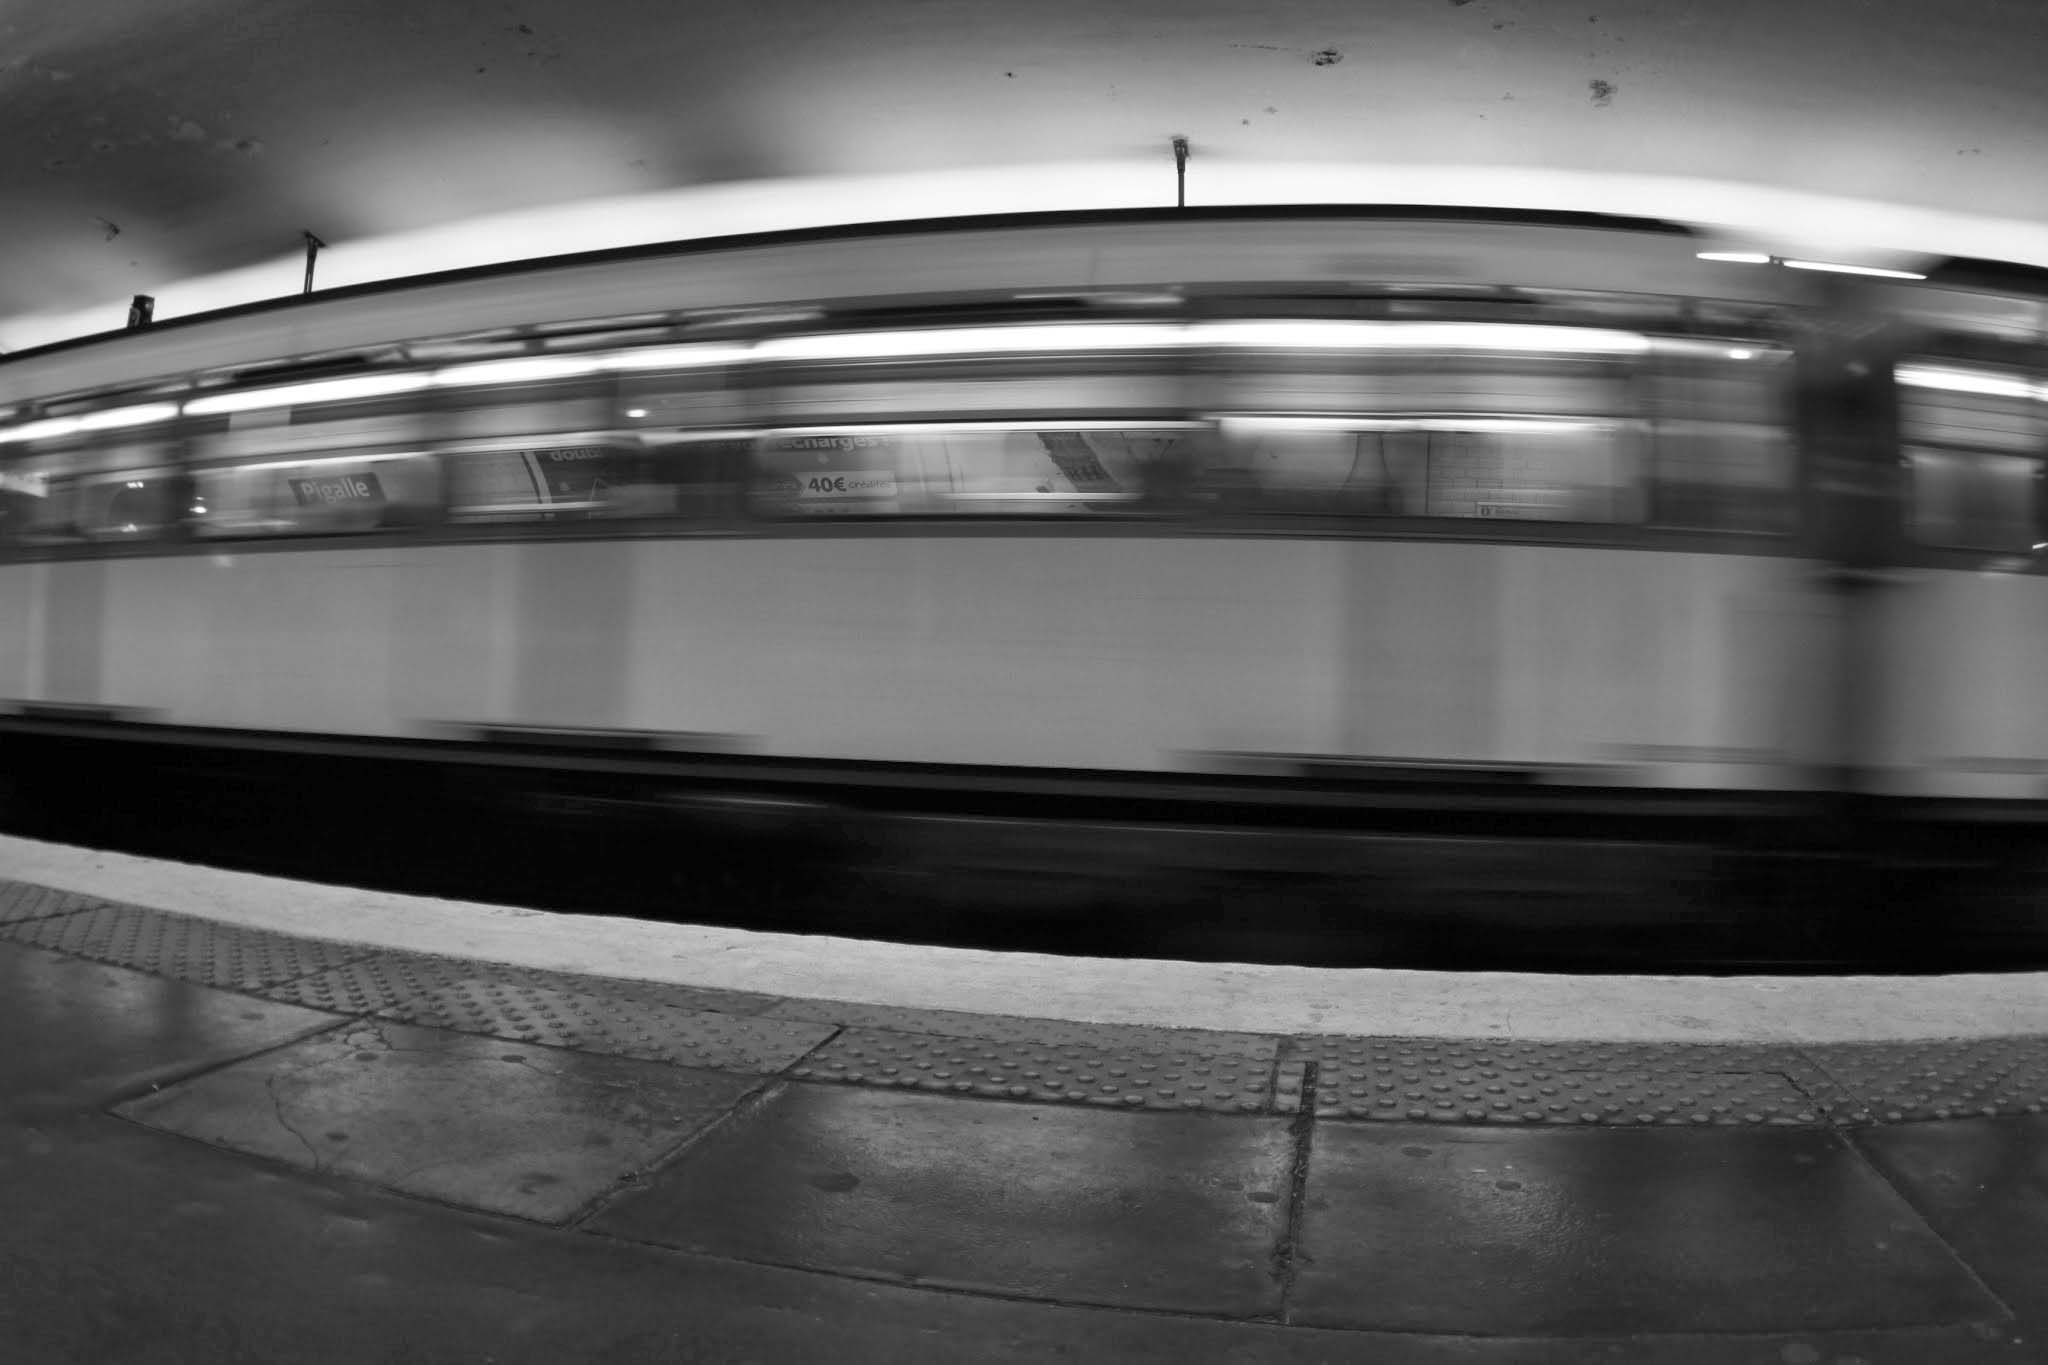
\includegraphics[height=\paperheight]{images/webforms_cover.jpg}
            };
        \end{tikzpicture}
     \end{frame}
}

%------------------------------------------------

\begin{frame}[fragile]
\frametitle{Readme}

\begin{block}{\scriptsize License:}
\tiny
 \begin{itemize}
  \item[] Creative Commons Attribution-NonCommercial-ShareAlike 4.0 International License \\ 
  \url{http://creativecommons.org/licenses/by-nc-sa/4.0/}{}
 \end{itemize}
\end{block}

\begin{block}{\scriptsize You are free to:}
\tiny
 \begin{itemize}
  \item[] \textcolor{darkgray}{\textbf{Share}} --- \textcolor{gray}{copy and redistribute the material}
  \item[] \textcolor{darkgray}{\textbf{Adapt}} --- \textcolor{gray}{rebuild and transform the material}
 \end{itemize}
\end{block}

\vspace{2mm}
\begin{block}{\scriptsize Under the following conditions:}
\tiny
\begin{itemize}
 \item[] \textcolor{darkgray}{\textbf{Attribution}} --- \textcolor{gray}{You must give appropriate credit, provide a link to the license, and indicate if changes were made.}
 \item[] \textcolor{darkgray}{\textbf{NonCommercial}} --- \textcolor{gray}{You may not use this work for commercial purposes.}
 \item[] \textcolor{darkgray}{\textbf{Share Alike}} --- \textcolor{gray}{If you remix, transform, or build upon this 
 work, you must distribute your contributions under the same license to this one.}
\end{itemize}
\end{block}

\end{frame}

%------------------------------------------------

\begin{frame}
\frametitle{Lectures Menu}

\begin{columns}[t]
\begin{column}{0.1\textwidth}
%--- empty space ---%
\end{column}
\begin{column}{0.8\textwidth}
 \begin{block}{Slide Decks}
  \begin{enumerate}
   \item \textcolor{lightgray}{Introduction}
   \item \textcolor{lightgray}{Reading files from the Web}
   \item \textcolor{lightgray}{Basics of XML and HTML}
   \item \textcolor{lightgray}{Parsing XML / HTML content}
   \item \textcolor{lightgray}{Handling JSON data}
   \item \textcolor{lightgray}{HTTP basics and the RCurl package}
   \item \textbf{Getting data via Web Forms}
   \item \textcolor{lightgray}{Getting data via Web services}
   %\item \textcolor{lightgray}{Web Scraping Case Study}
  \end{enumerate}
 \end{block}
\end{column}
\begin{column}{0.1\textwidth}
%--- empty space ---%
\end{column}
\end{columns}

\end{frame}

%------------------------------------------------

\begin{frame}
 \begin{center}
  \Huge{\textcolor{mandarina}{Data via \\ Web Forms}}
 \end{center}
\end{frame}

%------------------------------------------------

\begin{frame}
\frametitle{Goal}

\begin{columns}[t]
\begin{column}{0.1\textwidth}
%--- empty space ---%
\end{column}
\begin{column}{0.8\textwidth}

\begin{block}{Web Forms ...}
The goal of the present slides is to show you \textbf{how to get data via web forms} with R
\end{block}

\end{column}
\begin{column}{0.1\textwidth}
%--- empty space ---%
\end{column}
\end{columns}

\end{frame}

%------------------------------------------------

\begin{frame}
\frametitle{Synopsis}

\begin{columns}[t]
\begin{column}{0.1\textwidth}
%--- empty space ---%
\end{column}
\begin{column}{0.8\textwidth}

\begin{block}{In a nutshell}
We'll cover the following topics:
\begin{itemize}
 \item Basics of HTML Forms
 \item HTTP requests in Web forms
 \item R package \code{"RHTMLForms"}
 \item How to use \code{"RCurl"} to query HTML Forms
 \item Case Studies
\end{itemize}
\end{block}

\end{column}
\begin{column}{0.1\textwidth}
%--- empty space ---%
\end{column}
\end{columns}

\end{frame}

%------------------------------------------------

\begin{frame}
\frametitle{Some References}

\begin{itemize}
 \item XML and Web Technlogies for Data Sciences with R \\
 \low{by Deb Nolan and Duncan Temple Lang}
 \item HTML Forms W3C Tutorial \\
 {\scriptsize \url{http://www.w3.org/TR/html401/interact/forms.html}}
 \item R Package \code{"RHTMLForms"} \\
 {\scriptsize \url{http://www.omegahat.org/RHTMLForms/}}
\end{itemize}

\end{frame}

%------------------------------------------------

\begin{frame}
 \begin{center}
  \Huge{\textcolor{mandarina}{HTML Forms}}
 \end{center}
\end{frame}

%------------------------------------------------

\begin{frame}[fragile]
\frametitle{Examples of HTML Forms}

\begin{center}
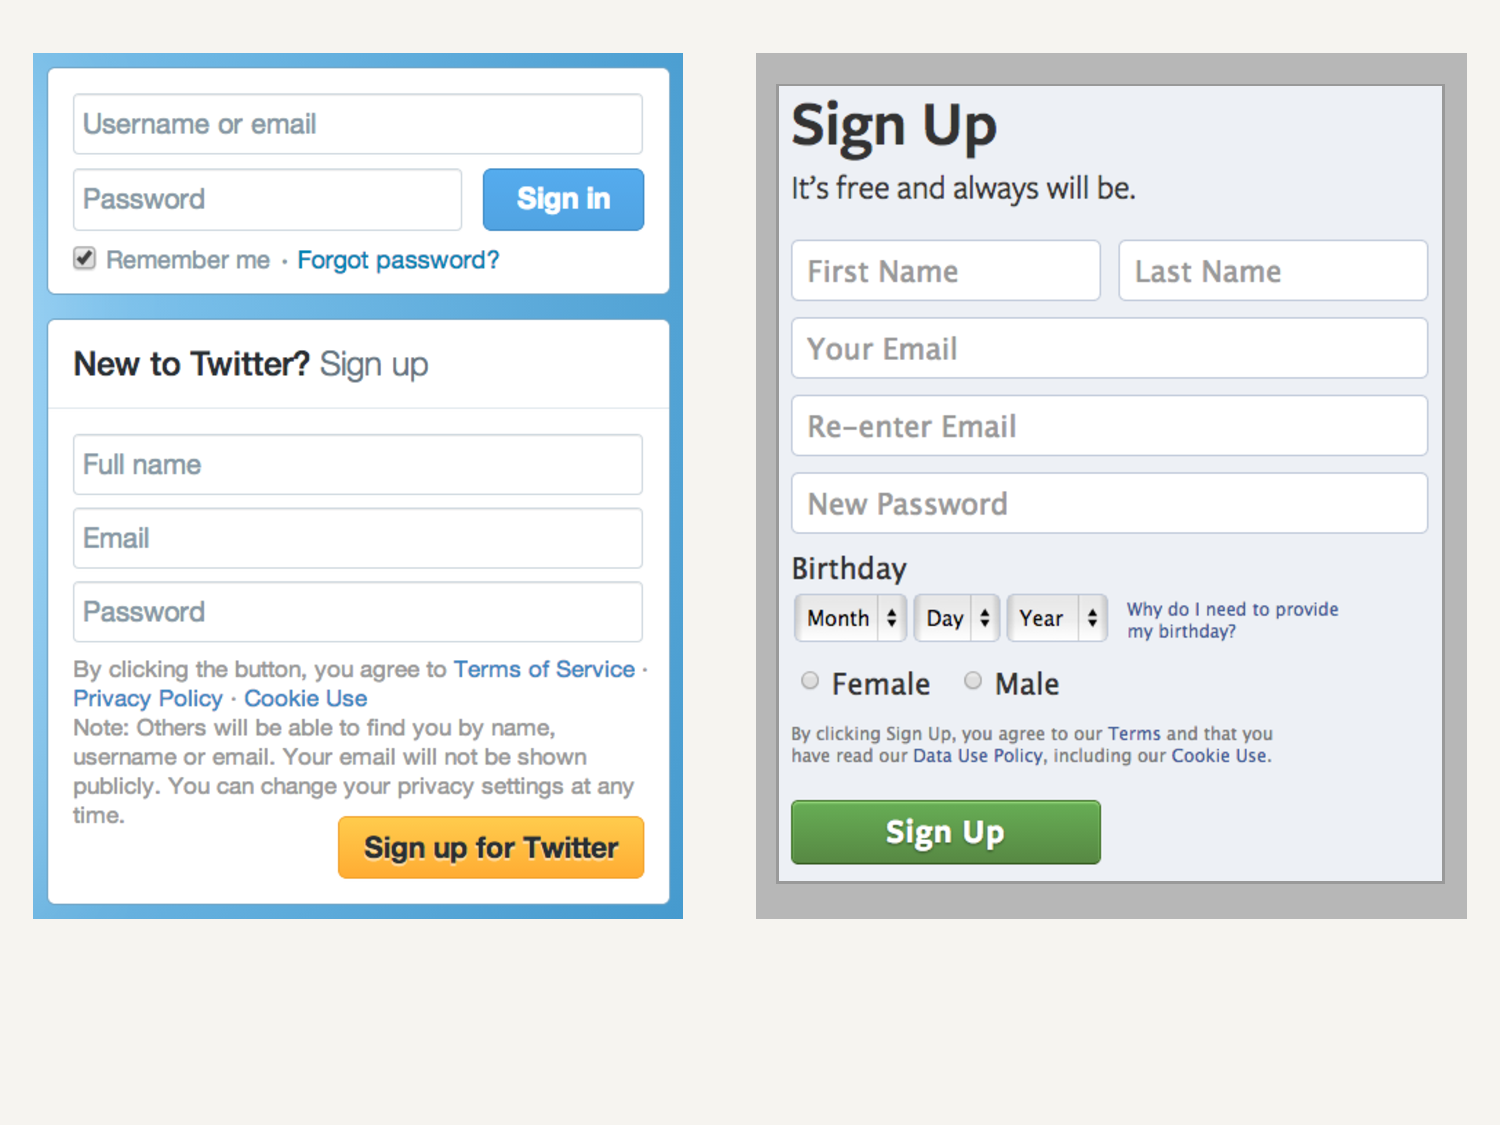
\includegraphics[width=10cm]{images/html_form_twitter_facebook.pdf}
\end{center}

\end{frame}

%------------------------------------------------

\begin{frame}[fragile]
\frametitle{Examples of HTML Forms}

\begin{center}
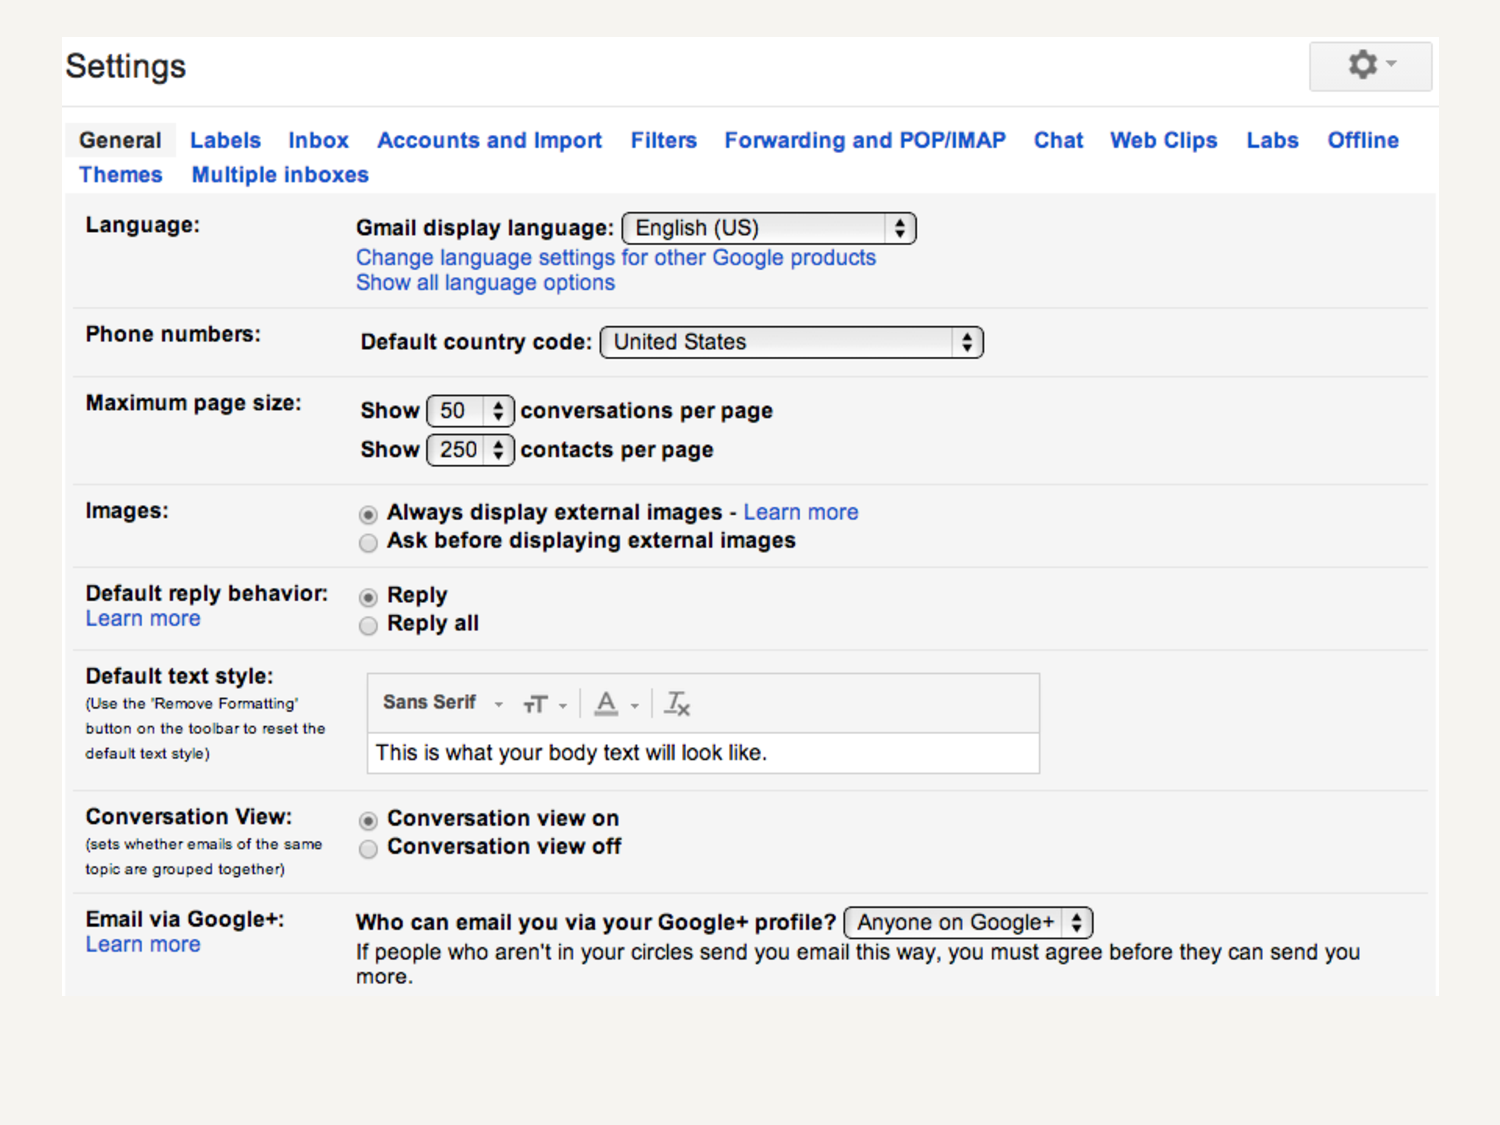
\includegraphics[width=11cm]{images/html_form_gmail.pdf}
\end{center}

\end{frame}

%------------------------------------------------

\begin{frame}[fragile]
\frametitle{HTML Forms?}

\begin{block}{HTML Forms?}
We use HTML Forms practically everyday: 
\begin{itemize}
 \item when we sign in to our email accounts
 \item when we make transactions online 
 \item when we post comments
 \item when we fill online surveys
 \item \textit{etc}
\end{itemize}
\end{block}

\end{frame}

%------------------------------------------------

\begin{frame}
\frametitle{HTML Forms}

\begin{columns}[t]
\begin{column}{0.1\textwidth}
%--- empty space ---%
\end{column}
\begin{column}{0.8\textwidth}

\begin{block}{HTML Forms \textit{(aka Web Forms)}:}
\begin{itemize}
 \item are used to gather information from the user
 \item transmit or \textit{submit} data to a server
 \item add interactivity to websites
\end{itemize}
\end{block}

\end{column}
\begin{column}{0.1\textwidth}
%--- empty space ---%
\end{column}
\end{columns}

\end{frame}

%------------------------------------------------

\begin{frame}[fragile]
\frametitle{Importance}

\begin{block}{Why should we care?}
Besides allowing websites to provide a way for interacting with users, HTML Forms play a prominent role regarding data on the Web.

\bigskip 

Admittedly, \textbf{large amounts of data on the Web are accessible via HTML Forms}. Hence the importance for being familiar with the basic concepts around Web Forms.
\end{block}

\end{frame}

%------------------------------------------------

\begin{frame}[fragile]
\frametitle{How Forms Work}

\begin{center}
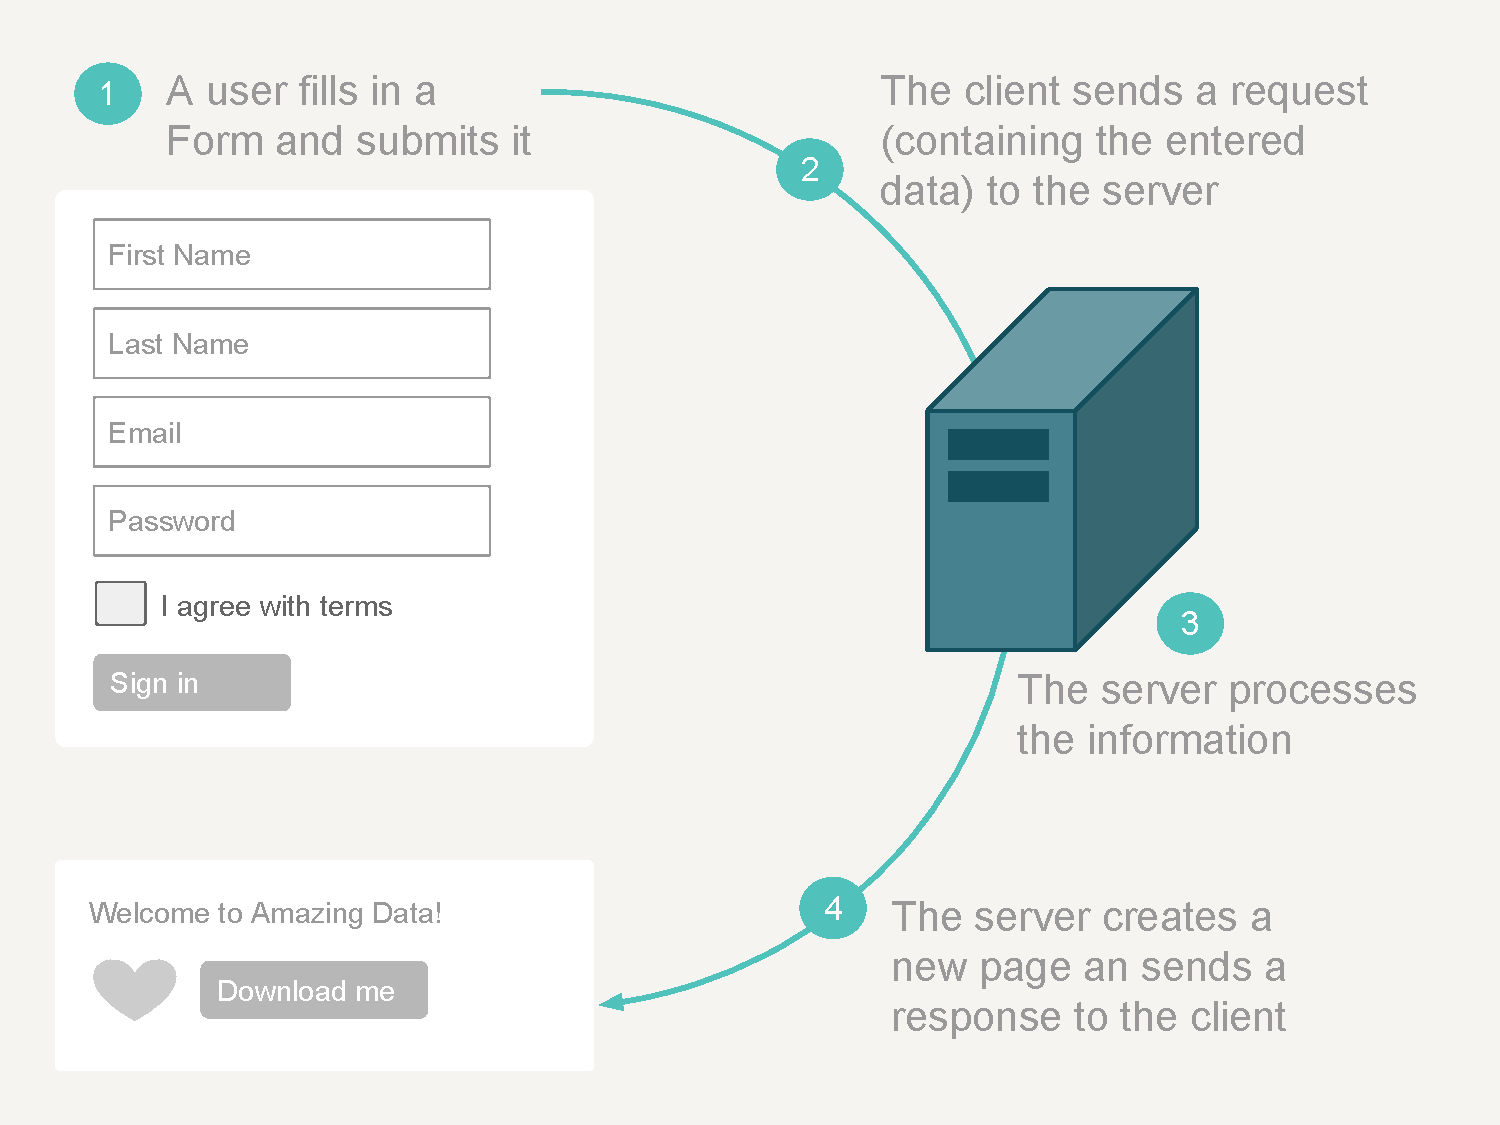
\includegraphics[width=10cm]{images/html_form_works.pdf}
\end{center}

\end{frame}

%------------------------------------------------

\begin{frame}[fragile]
\frametitle{HTML Forms}

\begin{block}{Broadly speaking ...}
Many websites have Forms that the visitors must use in order to provide some kind of input information.

\bigskip
This information is taken by the browser ---ie the client--- which submits a request to the server.

\bigskip
Based on the data submitted, the server takes an appropriate action and produces a customized response.
\end{block}

\end{frame}

%------------------------------------------------

\begin{frame}
 \begin{center}
  \Huge{\textcolor{mandarina}{Basics of HTML Forms}}
 \end{center}
\end{frame}

%------------------------------------------------

\begin{frame}[fragile]
\frametitle{HTML Form Element}

\begin{block}{Form Characteristics}
\begin{itemize}
 \item A Form is defined with an html \highcode{<form>} element. 
 \item A \code{<form>} element has 2 main attributes: \highcode{action} and \highcode{method}
 \item A \code{<form>} element is a container for all the content of the form
\end{itemize}
\end{block}

\begin{block}{Conceptual form}
\begin{verbatim}
  <form action="..." method="...">

     [The input elements go here]

  </form>
\end{verbatim}
\end{block}

\end{frame}

%------------------------------------------------

\begin{frame}
\frametitle{Form Action and Method}

\begin{block}{Form Attributes}
An HTML Form has 2 main attributes: \textbf{action} and \textbf{method}
\begin{itemize}
 \item the \highcode{action} attribute points to the server side script that handles the form submission
 \item the \highcode{method} defines the type of HTTP request that is used to submit the information: \code{GET} or \code{POST} 
\end{itemize}
\end{block}

\end{frame}

%------------------------------------------------

\begin{frame}[fragile]
\frametitle{HTML Forms}

\begin{block}{Form Controls}
\begin{itemize}
 \item The way Forms allow to capture input data is by using \textbf{form controls}
 \item Form controls live inside the \code{<form>} element
 \item There are several types of form controls \low{(eg text boxes, select menus, checkboxes, radio buttons, submit buttons)}
 \item Some of the more common controls are: 
 \begin{itemize}
  \item \code{<input>} \low{(there are various classes of inputs)}
  \item \code{<textarea>}
  \item \code{<select>}
  \item \code{<option>}
  \item \code{<button>}
 \end{itemize}
\end{itemize}
\end{block}

\end{frame}

%------------------------------------------------

\begin{frame}
\frametitle{Some HTML Form Controls}

\begin{center}
 \begin{tabular}{l l}
  \hline
  Control & Description \\
  \hline
  \code{<input type="text">} & text box \\
  \code{<input type="password">} & password box \\
  \code{<input type="radio">} &  radio button \\
  \code{<input type="checkbox">} & checkbox \\
  \code{<input type="submit">} & submit button \\
  \code{<input type="reset">} & reset button \\
  \code{<input type="hidden">} & hidden field \\
  \code{<input type="button">} & button \\
  \code{<select>} & selection \\
  \code{<option>} & selection \\
  \code{<textarea>} & text area \\
  \hline
 \end{tabular}
\end{center}

\end{frame}

%------------------------------------------------

\begin{frame}
\frametitle{Appearance of some Form Controls}

\begin{center}
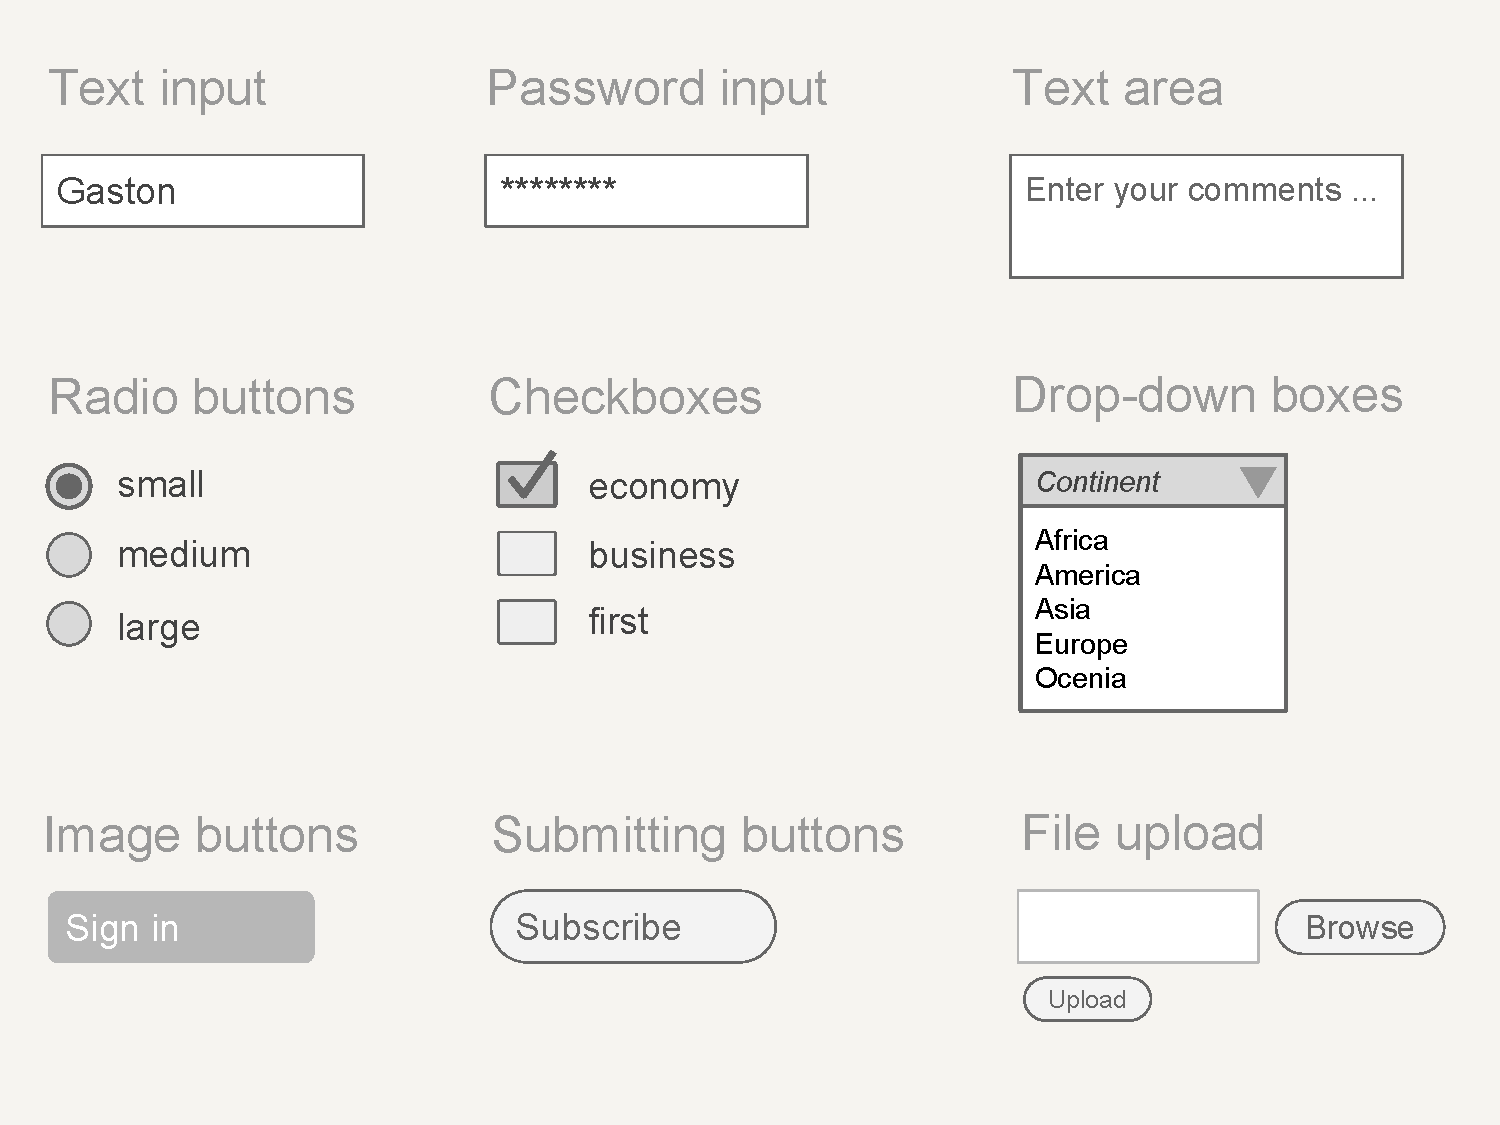
\includegraphics[width=11cm]{images/html_form_controls.pdf}
\end{center}

\end{frame}

%------------------------------------------------

\begin{frame}[fragile]
\frametitle{About Form Controls}

\begin{block}{Form Control Names}
The job of a form control is to gather one piece of information from the user. In order to uniquely identify the collected piece of data, controls have a \highcode{name} attribute.
\end{block}

\begin{block}{Control examples: Username and Password}
{\scriptsize
\begin{verbatim}
<form method="get" action="/bin/process">
    Enter your name: <input type="text" name="username"><br />
    Enter your password: <input type="password" name="password"><br />
</form>
\end{verbatim}
}
\end{block}
\end{frame}

%------------------------------------------------

\begin{frame}[fragile]
\frametitle{HTML Form in a Website}

\begin{center}
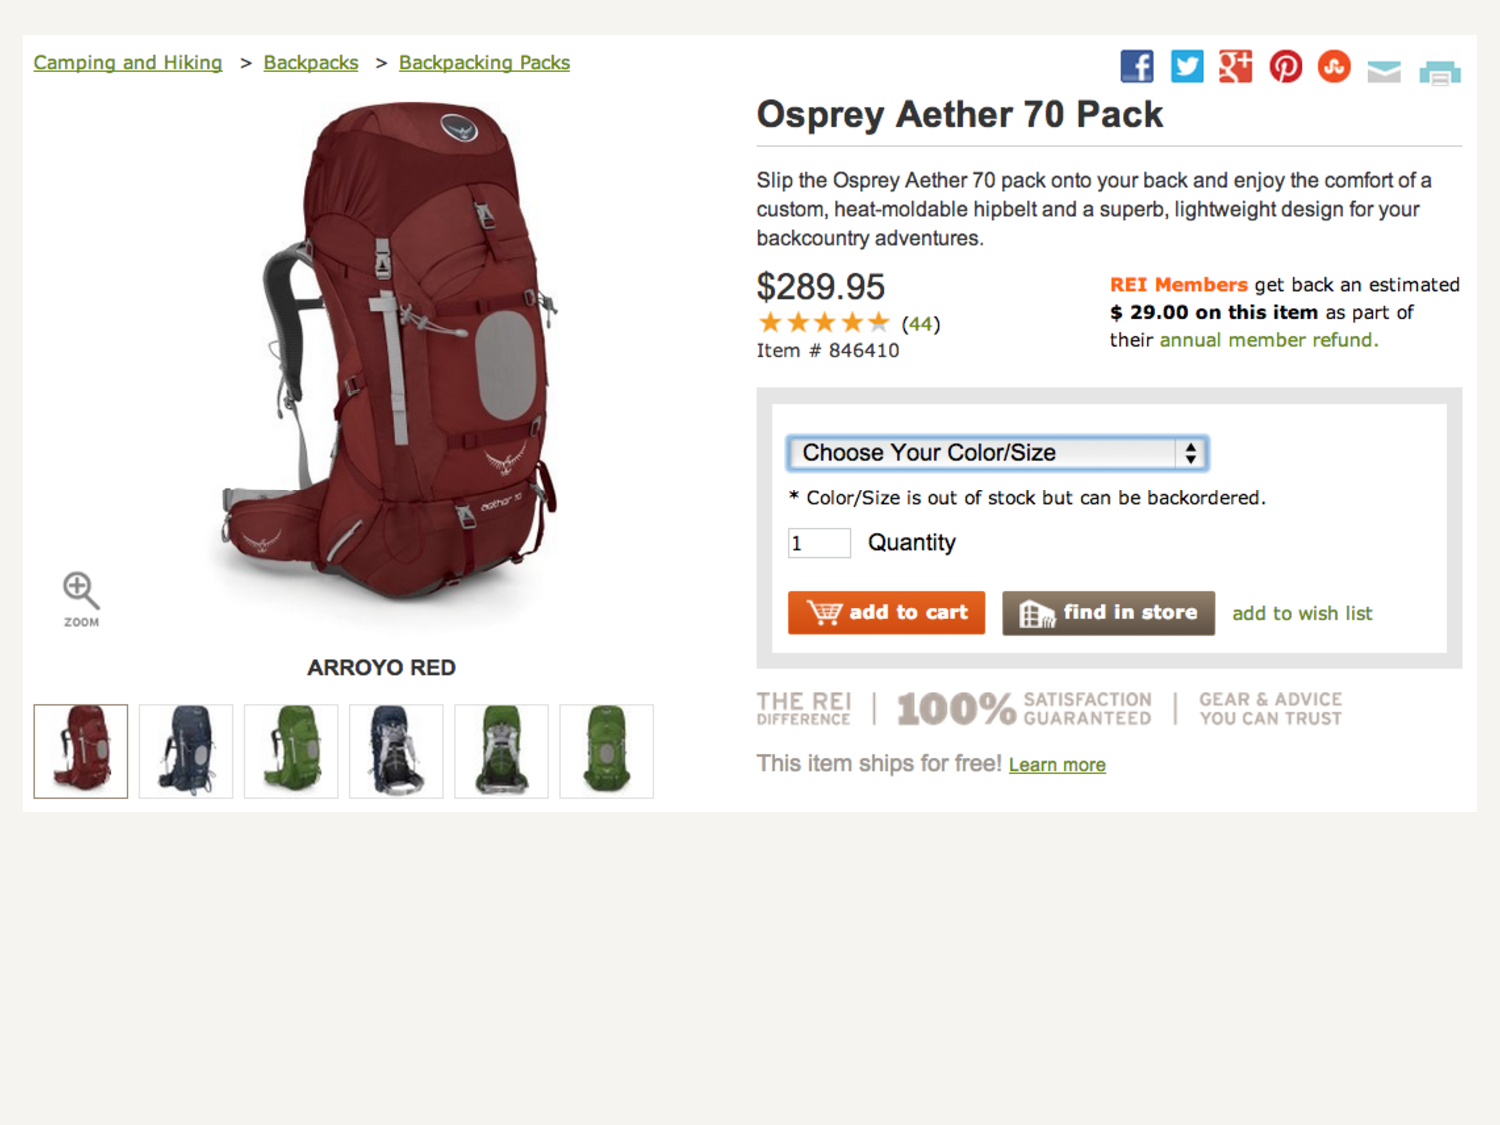
\includegraphics[width=11cm]{images/backpack_form.pdf}
\end{center}

\end{frame}

%------------------------------------------------

\begin{frame}[fragile]
\frametitle{HTML Form Components}

\begin{center}
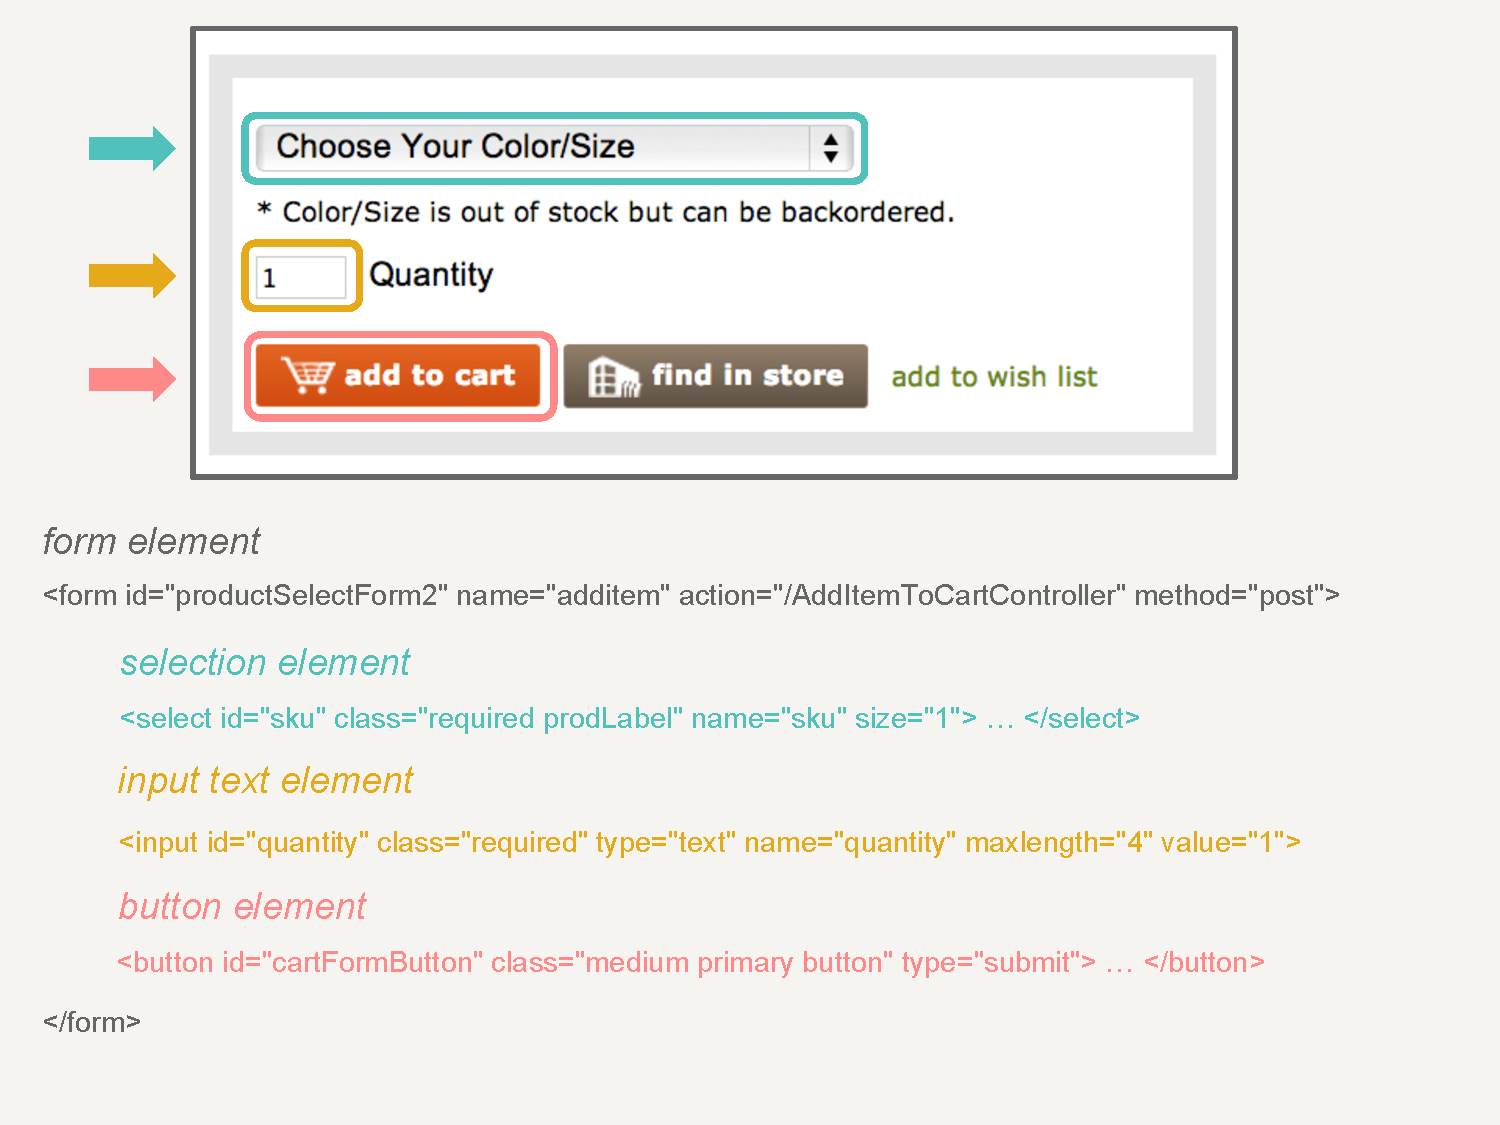
\includegraphics[width=11cm]{images/product_select.pdf}
\end{center}

\end{frame}

%------------------------------------------------

\begin{frame}
 \begin{center}
  \Huge{\textcolor{mandarina}{Submitting Forms}}
 \end{center}
\end{frame}

%------------------------------------------------

\begin{frame}
\frametitle{Form Submission}

\begin{block}{Submission Request}
Once the user fills in a Form and hits the submit button ---or any other type of submit action--- the browser gathers the input data and sends a request to the web browser. 
\end{block}

\begin{block}{HTTP Request Methods}
There are 2 \textit{requesting} mechanisms for submitting Web forms: 
\begin{itemize}
 \item using an \textbf{HTTP GET} request
 \item using an \textbf{HTTP POST} request
\end{itemize}
\end{block}

\end{frame}

%------------------------------------------------

\begin{frame}
\frametitle{Form Submission}

\begin{block}{HTTP Request Methods}
The type of request ---\code{GET} or \code{POST}--- depends on the \textbf{method} specified in the Web Form.
\end{block}

\begin{block}{Attribute \code{method}}
Remember that the HTTP request method is specified with the attribute \highcode{method} inside the \code{<form>} element.  
\end{block}

\end{frame}

%------------------------------------------------

\begin{frame}
\frametitle{Forms and HTTP Requests}

\begin{block}{HTTP methods in forms}
The way the browser gathers the input data is by collecting the \textbf{name} and \textbf{value} of each of the controls. We say that the browser packs them into \highcode{"name=value"} pairs.

\bigskip
Both methods, \code{GET} and \code{POST}, take the set of \code{name=value} pairs to parametrize the request.

\bigskip
The difference between \code{GET} and \code{POST} is in \textbf{how the name=value pairs are delivered to the Web server.}
\end{block}

\end{frame}

%------------------------------------------------

\begin{frame}[fragile]
\frametitle{Toy Example: Coffee Form}

\begin{center}
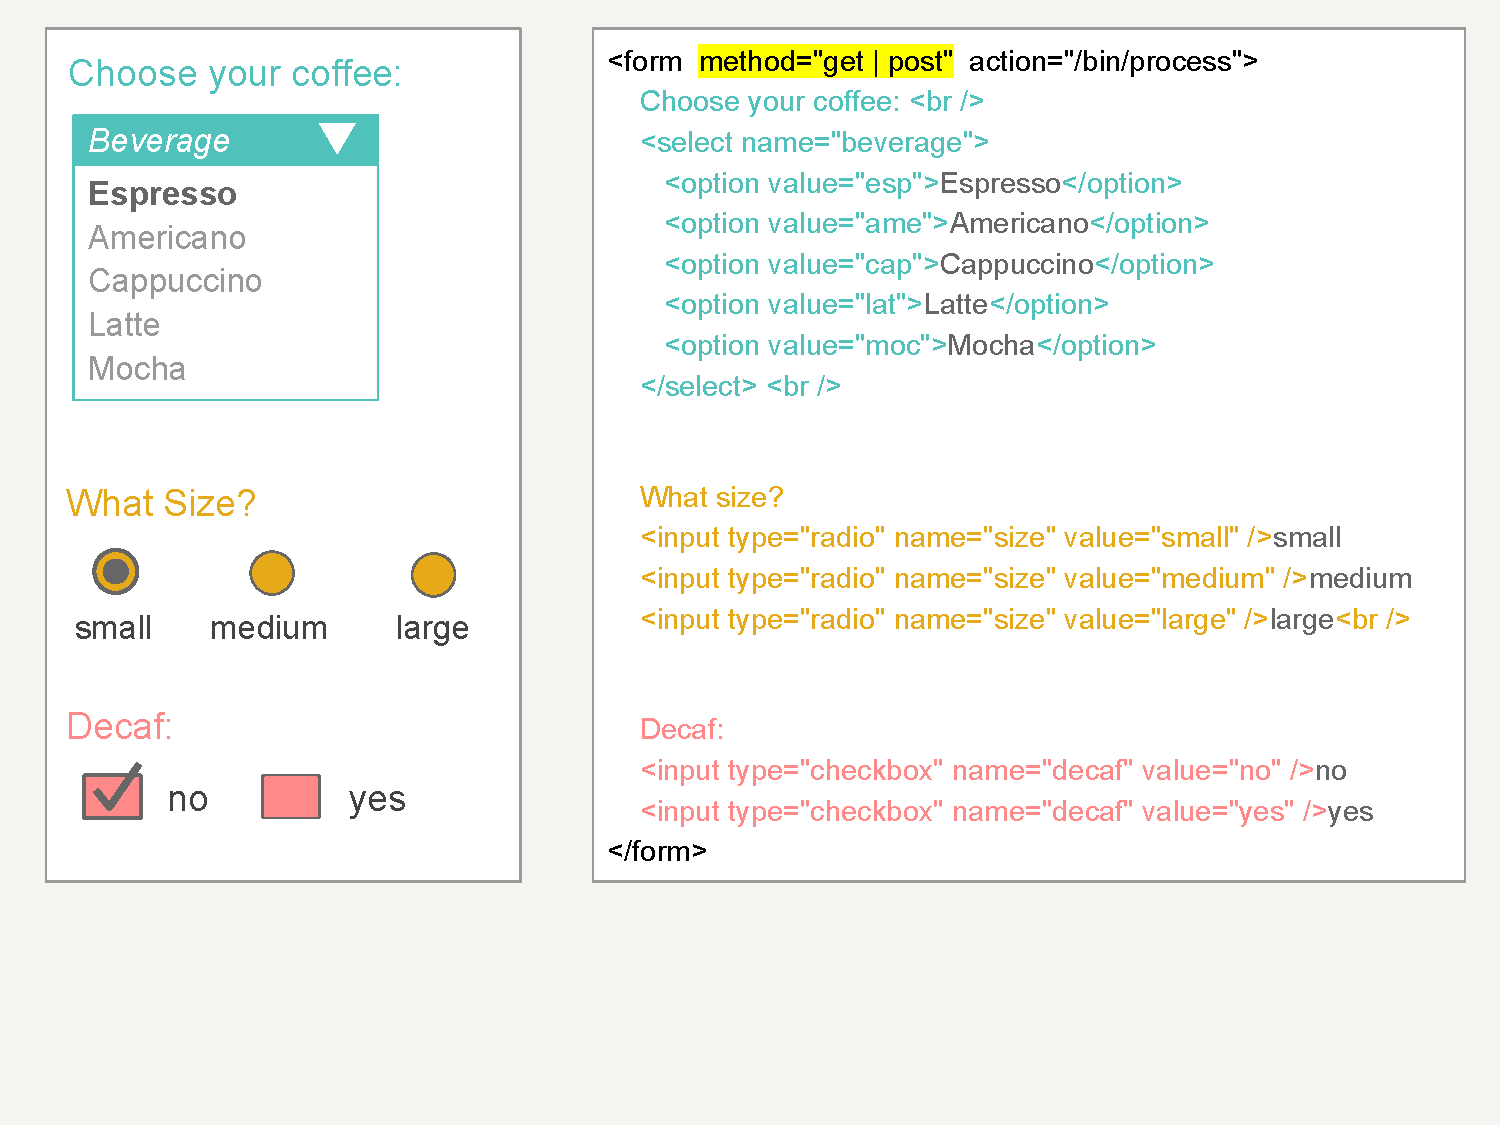
\includegraphics[width=11cm]{images/html_form_coffee.pdf}
\end{center}

\end{frame}

%------------------------------------------------

\begin{frame}[fragile]
\frametitle{Encoding of Name-Value Pairs}

\begin{block}{Name-Value Pairs}
The browser gathers the \textbf{name} and \textbf{value} of each of the control fields forming \highcode{name=value} pairs: 

\begin{itemize}
 \item \code{beverage=esp}
 \item \code{size=small}
 \item \code{decaf=no}
\end{itemize}
\end{block}

\begin{block}{Query String}
The \highcode{name=value} pairs are concatenated together into a \textbf{query string} using \highcode{"\&"} as a field separator: \\

\vspace{2mm}
\highcode{beverage=esp\&size=small\&decaf=no}
\end{block}

\end{frame}

%------------------------------------------------

\begin{frame}
\frametitle{Query String and Submit Methods}

\begin{block}{GET or POST}
The way the query string is handled depends on the request method:

\begin{itemize}
 \item If \code{GET} is used, name-value pairs are appended to the requested URL
 \item If \code{POST} is used, the name-value pairs are sent as part of the request body
\end{itemize}
\end{block}

\end{frame}

%------------------------------------------------

\begin{frame}[fragile]
\frametitle{Query String in GET and POST}

\begin{center}
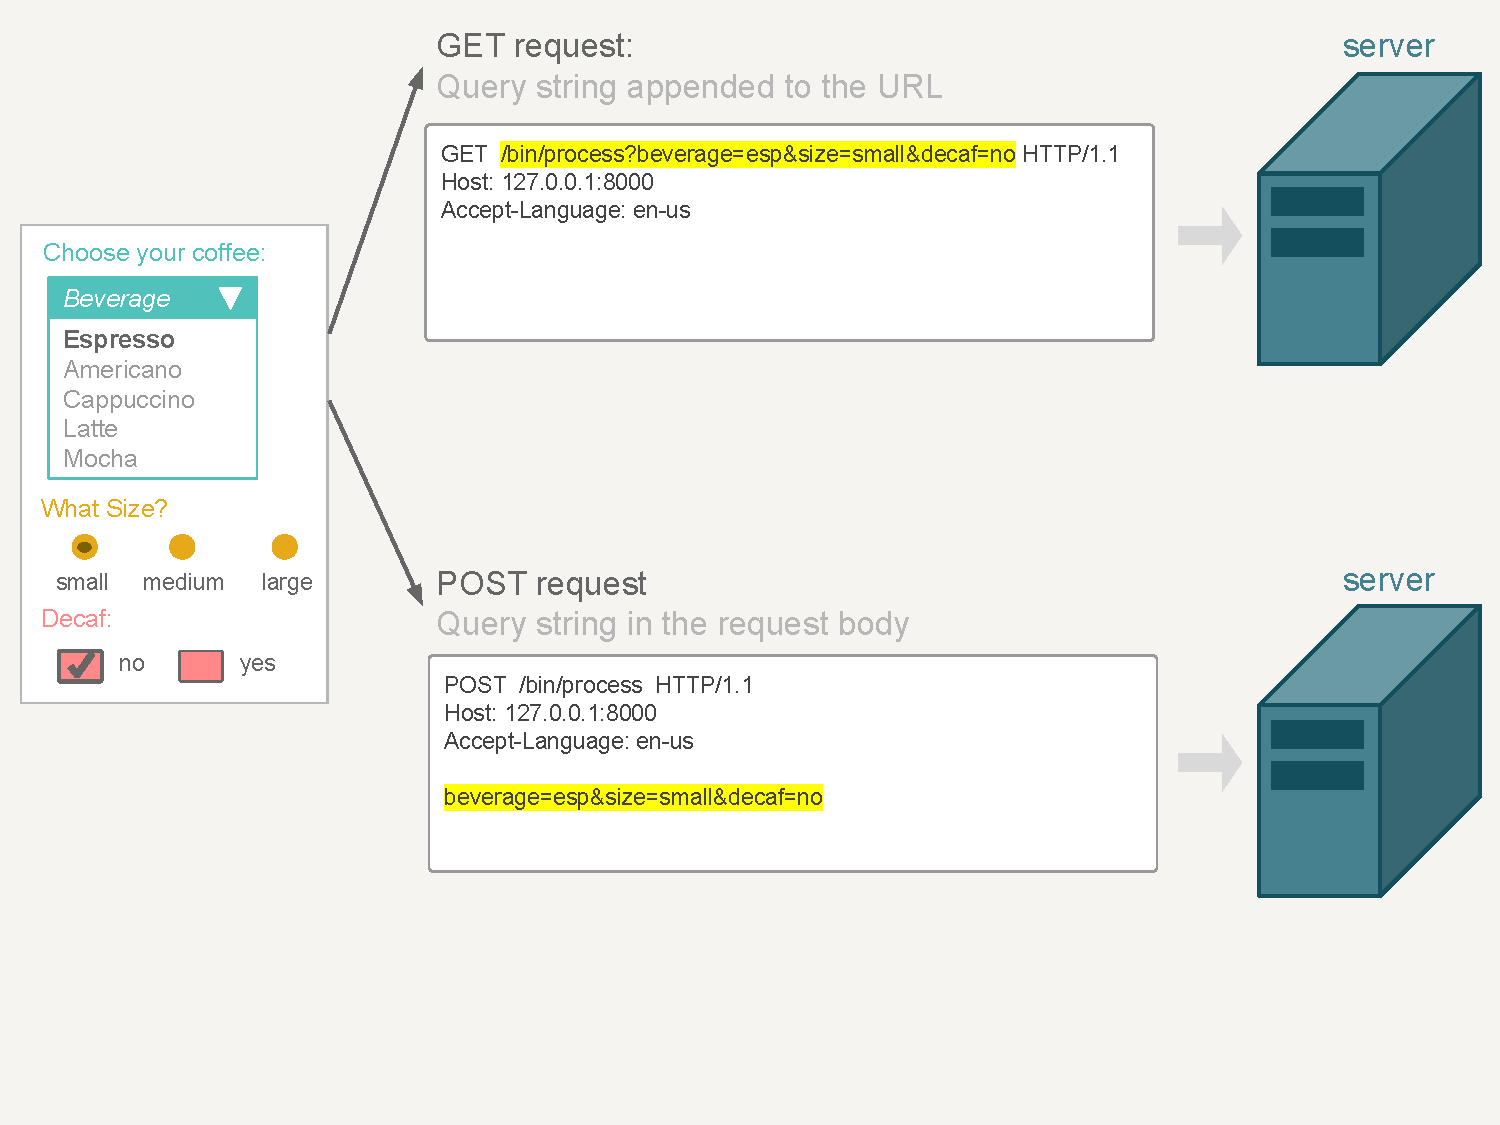
\includegraphics[width=11cm]{images/html_form_get_post.pdf}
\end{center}

\end{frame}

%------------------------------------------------

\begin{frame}[fragile]
\frametitle{GET Method}

\begin{block}{GET method}
With \code{GET}, the parameters are appended to the action and included as part of the URL in the HTTP request.
\end{block}

\begin{block}{Query string appended to URL}
{\footnotesize
\begin{verbatim}
GET /bin/process?beverage=esp&size=small&decaf=no HTTP/1.1
Host: 127.0.0.1:8000
Accept-Language: en-us
\end{verbatim}
}
\end{block}

\end{frame}

%------------------------------------------------

\begin{frame}[fragile]
\frametitle{POST Method}

\begin{block}{POST method}
With \code{POST}, the parameters are sent in the body of the HTTP request and the URL is simply the action
\end{block}

\begin{block}{Query string as part of the request body}
{\footnotesize
\begin{verbatim}
POST /bin/process HTTP/1.1
Host: 127.0.0.1:8000
Accept-Language: en-us

beverage=esp&size=small&decaf=no
\end{verbatim}
}
\end{block}

\end{frame}

%------------------------------------------------

\begin{frame}
 \begin{center}
  \Huge{\textcolor{mandarina}{R package \\ \code{"RHTMLForms"}}}
 \end{center}
\end{frame}

%------------------------------------------------

\begin{frame}
\frametitle{Package \code{RHTMLForms}}

\begin{block}{\code{RHTMLForms}}
There are several approaches to get data via Web Forms in R. One very nice way to do that is by using the package \code{"RHTMLForms"} \\
\low{(by Duncan Temple Lang)}
\end{block}

\begin{block}{What for?}
\highcode{"RHTMLForms"} is an ad-hoc package that allows us to interact with Web Forms in a simple manner without having to worry about all the overwhelming details behind the HTTP requests, the control fields, and the query strings.
\end{block}

\end{frame}

%------------------------------------------------

\begin{frame}[fragile]
\frametitle{Installing \code{RHTMLForms}}

\begin{block}{Package Source}
At the moment of this writing, \code{"RHTMLForms"} is NOT available on CRAN. Instead, the package must be downloaded from: \\
{\footnotesize \url{http://www.omegahat.net/RHTMLForms/}}

\bigskip

For these slides I'm using the package version \code{0.6-0} from the source file ---\textit{tarball}--- \highcode{RHTMLForms\_0.6-0.tar.gz}

\bigskip

\low{Once you downloaded the package \code{tar.gz} file, you can proceed with the installation in R.}
\end{block}

\end{frame}

%------------------------------------------------

\begin{frame}[fragile]
\frametitle{Installing \code{RHTMLForms}}

\begin{block}{Installation}
Let's assume the \textit{tarball} file \highcode{RHTMLForms\_0.6-0.tar.gz} is in your \code{Downloads} directory. 

\bigskip

To install \code{"RHTMLForms"} in R type the following in your console:
\begin{knitrout}\footnotesize
\definecolor{shadecolor}{rgb}{1, 1, 1}\color{fgcolor}\begin{kframe}
\begin{alltt}
\hlcom{# installing RHTMLForms}
\hlkwd{install.packages}\hlstd{(}\hlstr{"~/Downloads/RHTMLForms_0.6-0.tar.gz"}\hlstd{,}
                 \hlkwc{repos} \hlstd{=} \hlkwa{NULL}\hlstd{,} \hlkwc{type} \hlstd{=} \hlstr{"source"}\hlstd{)}
\end{alltt}
\end{kframe}
\end{knitrout}
\end{block}

\end{frame}

%------------------------------------------------

\begin{frame}
\frametitle{Working with HTML Forms}

\begin{block}{Preliminaries}
Getting data via HTML Forms requires you to understand the type of Forms you are interacting with: 
\begin{itemize}
 \item what method the Forms use (\code{GET} or \code{POST})
 \item what control inputs they have (buttons, text, etc)
 \item what type of output is produced by the Server
\end{itemize}
\end{block}

\end{frame}

%------------------------------------------------

\begin{frame}
\frametitle{Working with HTML Forms}

\begin{block}{Preliminaries}
There's a \textit{workflow procedure} that we should follow to take full advantage of \code{"RHTMLForms"}: 
\begin{enumerate}
 \item we start by \textbf{exploring the website} that contains the Forms \\
 \low{(how many forms, what structure they have, etc)}
 \item we get a \textbf{description} of the Forms we are interested in
 \item we \textbf{figure out what inputs} we need to pass to the Forms
 \item we \textbf{submit} the necessary requests
 \item we \textbf{process} the documents produced by the Server
\end{enumerate}
\end{block}

\end{frame}

%------------------------------------------------

\begin{frame}[fragile]
\frametitle{Using RHTMLForms}

\begin{center}
Let's start with the Google search form


\includegraphics[width=10cm]{images/html_form_google.pdf}
\end{center}

\end{frame}

%------------------------------------------------

\begin{frame}[fragile]
\frametitle{Google Search Form}

\begin{block}{Structure of the Google Search Form}
If you oepn your \textit{web inspection tool} or see the source code of Google's Search homepage, you should be able to identify the HTML form:
\end{block}

{\scriptsize
\begin{verbatim}
<form action="/search" id="f" method="get">
  <div id="hf"></div>
  <div id="fkbx">
    <input id="q" jsaction="mousedown:ntp.fkbxclk" aria-hidden="true" 
     autocomplete="off" name="q" tabindex="-1" style="opacity: 0;">
    <div id="fkbx_crt"></div>
    <div id="fkbx-spch" tabindex="1" aria-label="Search by voice"
     style="display: block;"></div>
    <div id="fkbx-hspch" tabindex="1" aria-label="Listening for "Ok Google"">
    </div>
    <div id="fkbx-hht">Say "Ok Google"</div>    
  </div>
</form>
\end{verbatim}
}

\end{frame}

%------------------------------------------------

\begin{frame}[fragile]
\frametitle{\code{getHTMLFormDescription()}}

The main function to \textit{explore} the Forms in a website is \highcode{getHTMLFormDescription()} which allows us to process an HTML document and get a description of its Forms:

\begin{columns}[t]
\begin{column}{0.5\textwidth}
\begin{knitrout}\tiny
\definecolor{shadecolor}{rgb}{1, 1, 1}\color{fgcolor}\begin{kframe}
\begin{alltt}
\hlcom{# load RHTMLForms}
\hlkwd{library}\hlstd{(RHTMLForms)}

\hlcom{# google url}
\hlstd{google} \hlkwb{=} \hlstr{"http://www.google.com"}

\hlcom{# get forms}
\hlstd{google_forms} \hlkwb{=} \hlkwd{getHTMLFormDescription}\hlstd{(google)}

\hlstd{google_forms}
\end{alltt}
\begin{verbatim}
## $f
## HTML Form: http://www.google.com/search 
## q: [  ]
\end{verbatim}
\end{kframe}
\end{knitrout}

In this case there's only one form: \highcode{q} (which is a query search)
\end{column}

\begin{column}{0.5\textwidth}
\begin{knitrout}\tiny
\definecolor{shadecolor}{rgb}{1, 1, 1}\color{fgcolor}\begin{kframe}
\begin{alltt}
\hlcom{# put the form in a separate object}
\hlstd{gform} \hlkwb{=} \hlstd{google_forms}\hlopt{$}\hlstd{f}

\hlcom{# object attributes}
\hlkwd{attributes}\hlstd{(gform)}
\end{alltt}
\begin{verbatim}
## $names
## [1] "formAttributes" "elements"       "url"           
## 
## $class
## [1] "HTMLFormDescription"
\end{verbatim}
\end{kframe}
\end{knitrout}

Note that the \code{gform} is of class \code{"HTMLFormDescription"}
\end{column}
\end{columns}

\end{frame}

%------------------------------------------------

\begin{frame}[fragile]
\frametitle{\code{getHTMLFormDescription()}}

We can obtain a number of descriptive features from an object of class \highcode{"HTMLFormDescription"}:

\begin{columns}[t]
\begin{column}{0.5\textwidth}
\begin{knitrout}\tiny
\definecolor{shadecolor}{rgb}{1, 1, 1}\color{fgcolor}\begin{kframe}
\begin{alltt}
\hlcom{# form attributes}
\hlstd{gform}\hlopt{$}\hlstd{formAttributes}
\end{alltt}
\begin{verbatim}
##                         action                           name 
## "http://www.google.com/search"                            "f" 
##                         method 
##                          "get" 
## attr(,"class")
## [1] "HTMLFormAttributes"
\end{verbatim}
\begin{alltt}
\hlcom{# form url}
\hlstd{gform}\hlopt{$}\hlstd{url}
\end{alltt}
\begin{verbatim}
##                         action 
## "http://www.google.com/search"
\end{verbatim}
\end{kframe}
\end{knitrout}
\end{column}

\begin{column}{0.5\textwidth}
\begin{knitrout}\tiny
\definecolor{shadecolor}{rgb}{1, 1, 1}\color{fgcolor}\begin{kframe}
\begin{alltt}
\hlcom{# form elements}
\hlstd{gform}\hlopt{$}\hlstd{elements}
\end{alltt}
\begin{verbatim}
## $ie
## ie: ISO-8859-1
## 
## $hl
## hl: en
## 
## $source
## source: hp
## 
## $biw
## biw: 
## 
## $bih
## bih: 
## 
## $q
## q: [  ]  
## 
## $gbv
## gbv: 1
## 
## attr(,"class")
## [1] "HTMLFormElementsList"
\end{verbatim}
\end{kframe}
\end{knitrout}
\end{column}
\end{columns}

\end{frame}

%------------------------------------------------

\begin{frame}
\frametitle{Working with \code{getHTMLFormDescription()}}

\begin{block}{What does \code{getHTMLFormDescription()} do?}
\begin{itemize}
 \item parses an HTML document and processes each \highcode{<form>} element
 \item returns a list containing the identified \code{<form>}'s
 \item each list element is of class \highcode{"HTMLFormDescription"}
 \item determines the URL to which we should submit the form
 \item identifies the method for submitting the form (\code{GET}, \code{POST})
\end{itemize}
\end{block}

\begin{block}{For each \code{"HTMLFormDescription"} element we can check}
\begin{itemize}
 \item \highcode{\$formAttributes}
 \item \highcode{\$elements}
 \item \highcode{\$url}
\end{itemize}
\end{block}

\end{frame}

%------------------------------------------------

\begin{frame}
\frametitle{\code{createFunction()}}

\begin{block}{\code{createFunction()}}
There's a very handy function called \highcode{createFunction()} that we can use on each of the elements \code{"HTMLFormDescription"}

\bigskip

\highcode{createFunction()} generates an R function for \textbf{form submission}. Together with the package \code{"RCurl"}, \code{createFunction()} allows us to specify values for each of the Form parameters, and obtain the result from the Web server.
\end{block}

\end{frame}

%------------------------------------------------

\begin{frame}[fragile]
\frametitle{\code{getHTMLFormDescription()}}

\highcode{createFunction()} allows us to create an R function to generate our own \textit{Google Search Form Submission}. 
\begin{knitrout}\tiny
\definecolor{shadecolor}{rgb}{1, 1, 1}\color{fgcolor}\begin{kframe}
\begin{alltt}
\hlcom{# create submitting function for google search Form}
\hlstd{google_submit} \hlkwb{=} \hlkwd{createFunction}\hlstd{(gform)}
\end{alltt}
\end{kframe}
\end{knitrout}

With the created function, and using \code{"RCurl"}, we can submit a search Form. Then we can parse the obtained outcome with one of the functions from \code{"XML"}:
\begin{knitrout}\tiny
\definecolor{shadecolor}{rgb}{1, 1, 1}\color{fgcolor}\begin{kframe}
\begin{alltt}
\hlcom{# load RCurl}
\hlkwd{library}\hlstd{(RCurl)}

\hlcom{# submit a search of the term "R project"}
\hlstd{r_project} \hlkwb{=} \hlkwd{google_submit}\hlstd{(}\hlstr{"R project"}\hlstd{)}

\hlcom{# we can then parse the content}
\hlkwd{library}\hlstd{(XML)}
\hlstd{r_project} \hlkwb{=} \hlkwd{htmlParse}\hlstd{(r_project)}
\end{alltt}
\end{kframe}
\end{knitrout}

\end{frame}

%------------------------------------------------

\begin{frame}
 \begin{center}
  \Huge{\textcolor{mandarina}{Case Study: \\ National Parks}}
 \end{center}
\end{frame}

%------------------------------------------------

{ % all template changes are local to this group.
    \setbeamertemplate{navigation symbols}{}
    \begin{frame}[plain]
        \begin{tikzpicture}[remember picture,overlay]
            \node[at=(current page.center)] {
                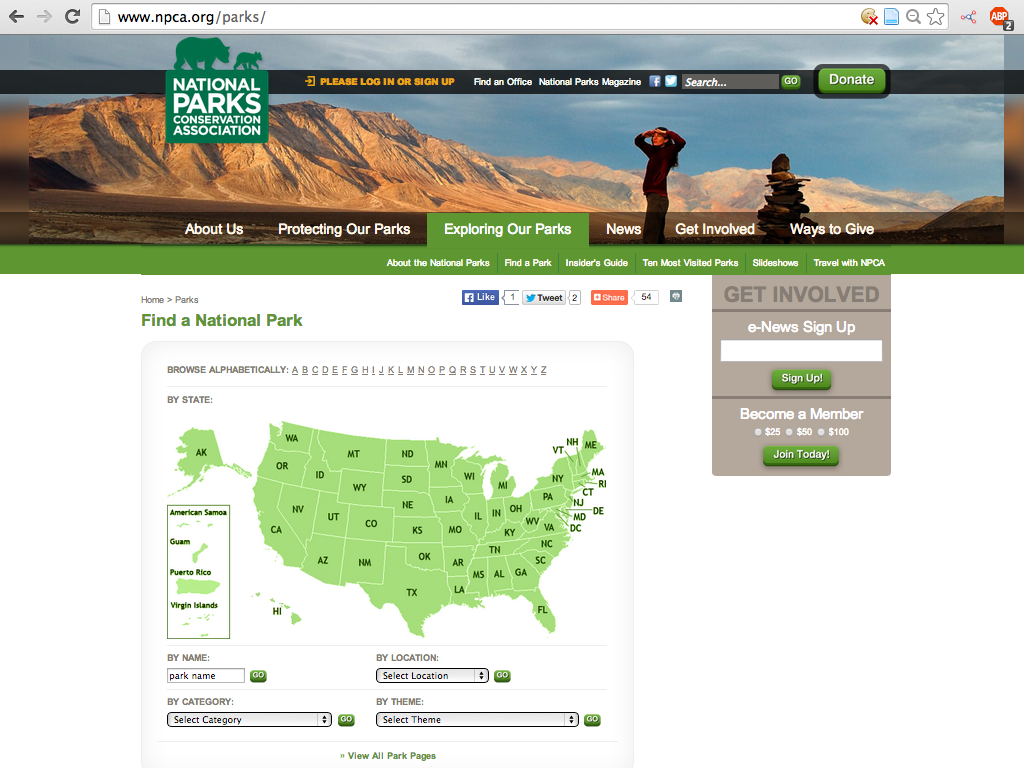
\includegraphics[width=\paperwidth]{images/national_parks_site.png}
            };
        \end{tikzpicture}
     \end{frame}
}

%------------------------------------------------

\begin{frame}
\frametitle{National Parks Conservation Association}

\begin{block}{NPCA}
The website of the \textit{National Parks Conservation Association} (NPCA) has a page that allows us to find a National Park: \\
{\footnotesize \url{http://www.npca.org/parks/}}
\end{block}

\begin{block}{What for}
Let's use \code{"RHTMLForms"} to get information and descriptions about the forms available in the \textit{Find a National Park} page.
\end{block}

\end{frame}

%------------------------------------------------

\begin{frame}[fragile]
\frametitle{Finding a National Park}

Let's start with \highcode{getHTMLFormDescription()} to get the list of form descriptions:

\begin{knitrout}\tiny
\definecolor{shadecolor}{rgb}{1, 1, 1}\color{fgcolor}\begin{kframe}
\begin{alltt}
\hlcom{# npca url}
\hlstd{npca} \hlkwb{=} \hlstr{"http://www.npca.org/parks"}

\hlcom{# get descriptions of forms}
\hlstd{park_forms} \hlkwb{=} \hlkwd{getHTMLFormDescription}\hlstd{(npca)}

\hlcom{# how many forms}
\hlkwd{length}\hlstd{(park_forms)}
\end{alltt}
\end{kframe}
\end{knitrout}

\begin{knitrout}\tiny
\definecolor{shadecolor}{rgb}{1, 1, 1}\color{fgcolor}\begin{kframe}
\begin{verbatim}
## [1] 10
\end{verbatim}
\end{kframe}
\end{knitrout}

\low{We are interested in the Forms that have to do with \textit{Finding a National Park}}
\end{frame}

%------------------------------------------------

\begin{frame}[fragile]
\frametitle{Inspecting NPCA Forms}

The first three Forms are NOT the ones we want:
\begin{knitrout}\tiny
\definecolor{shadecolor}{rgb}{1, 1, 1}\color{fgcolor}\begin{kframe}
\begin{alltt}
\hlcom{# 1st form (not interesting)}
\hlstd{park_forms[[}\hlnum{1}\hlstd{]]}
\end{alltt}
\begin{verbatim}
## HTML Form: /search-results.html 
## q: [ Search... ]
\end{verbatim}
\begin{alltt}
\hlcom{# 2nd form (not interesting)}
\hlstd{park_forms[[}\hlnum{2}\hlstd{]]}
\end{alltt}
\begin{verbatim}
## HTML Form: http://npca.convio.net/site/Survey 
## cons_email: [  ]
\end{verbatim}
\begin{alltt}
\hlcom{# 3rd form (not interesting)}
\hlstd{park_forms[[}\hlnum{3}\hlstd{]]}
\end{alltt}
\begin{verbatim}
## HTML Form: http://my.npca.org/site/Donation2?df_id=1333&Level=1716&1333.donation=form1&s_subsrc=sidebar_nologin 
## donation_amount: on
\end{verbatim}
\end{kframe}
\end{knitrout}

\end{frame}

%------------------------------------------------

\begin{frame}[fragile]
\frametitle{Inspecting NPCA Forms}

The 4th Form does have to do with \textit{Finding a National Park}
\begin{knitrout}\tiny
\definecolor{shadecolor}{rgb}{1, 1, 1}\color{fgcolor}\begin{kframe}
\begin{alltt}
\hlcom{# 4th form (now we're talking)}
\hlstd{park_forms[[}\hlnum{4}\hlstd{]]}
\end{alltt}
\begin{verbatim}
## HTML Form: /exploring-our-parks/parks/search.jsp 
## query: [ park name ]
\end{verbatim}
\begin{alltt}
\hlcom{# park name form}
\hlstd{park_name} \hlkwb{=} \hlstd{park_forms[[}\hlnum{4}\hlstd{]]}

\hlcom{# form attributes}
\hlstd{park_name}\hlopt{$}\hlstd{formAttributes}
\end{alltt}
\begin{verbatim}
##                                  action 
## "/exploring-our-parks/parks/search.jsp" 
##                                  method 
##                                   "get" 
## attr(,"class")
## [1] "HTMLFormAttributes"
\end{verbatim}
\end{kframe}
\end{knitrout}

This is a \textbf{query} input that uses a \code{GET} method

\end{frame}

%------------------------------------------------

\begin{frame}[fragile]
\frametitle{Park State Form}

Let's get the 5th form in a separate object before creating a submission form function:

\begin{knitrout}\tiny
\definecolor{shadecolor}{rgb}{1, 1, 1}\color{fgcolor}\begin{kframe}
\begin{alltt}
\hlcom{# 5th form (park state form)}
\hlstd{park_state} \hlkwb{=} \hlstd{park_forms[[}\hlnum{5}\hlstd{]]}
\hlstd{park_state}\hlopt{$}\hlstd{elements}
\end{alltt}
\begin{verbatim}
## $state
## state: [  ]  , al, ak, as, az, ar, ca, co, ct, de, dc, fl, ga, gu, hi, id, il, in, ia, ks, ky, la, me, md, ma, mi, mn, ms, mo, mt, ne, nv, nh, nj, nm, ny, nc, nd, oh, ok, or, pa, pr, ri, mp, sc, sd, tn, tx, ut, vt, vi, va, wa, wv, wi, wy, Select Location, Alabama, Alaska, American Samoa, Arizona, Arkansas, California, Colorado, Connecticut, Delaware, District of Columbia, Florida, Georgia, Guam, Hawaii, Idaho, Illinois, Indiana, Iowa, Kansas, Kentucky, Louisiana, Maine, Maryland, Massachusetts, Michigan, Minnesota, Mississippi, Missouri, Montana, Nebraska, Nevada, New Hampshire, New Jersey, New Mexico, New York, North Carolina, North Dakota, Ohio, Oklahoma, Oregon, Pennsylvania, Puerto Rico, Rhode Island, Saipan, South Carolina, South Dakota, Tennessee, Texas, Utah, Vermont, Virgin Islands, Virginia, Washington State, West Virginia, Wisconsin, Wyoming
## 
## attr(,"class")
## [1] "HTMLFormElementsList"
\end{verbatim}
\begin{alltt}
\hlstd{park_state}\hlopt{$}\hlstd{formAttributes}
\end{alltt}
\begin{verbatim}
##                                      action 
## "/exploring-our-parks/parks/park-list.html" 
##                                      method 
##                                       "get" 
## attr(,"class")
## [1] "HTMLFormAttributes"
\end{verbatim}
\end{kframe}
\end{knitrout}

\end{frame}

%------------------------------------------------

\begin{frame}[fragile]
\frametitle{Park State Form}

Here's how to create a submission form function for the Park State Form:

\begin{knitrout}\tiny
\definecolor{shadecolor}{rgb}{1, 1, 1}\color{fgcolor}\begin{kframe}
\begin{alltt}
\hlkwd{require}\hlstd{(RCurl)}

\hlcom{# create 'form submission' function for park state}
\hlstd{park_state_fun} \hlkwb{=} \hlkwd{createFunction}\hlstd{(park_state)}

\hlcom{# submission for parks in California}
\hlstd{cal_parks} \hlkwb{=} \hlkwd{park_state_fun}\hlstd{(}\hlstr{"California"}\hlstd{)}
\end{alltt}
\end{kframe}
\end{knitrout}

Finally, we can use the \highcode{getHTMLLinks()} function from \code{"XML"} to extract all the links:

\begin{knitrout}\tiny
\definecolor{shadecolor}{rgb}{1, 1, 1}\color{fgcolor}\begin{kframe}
\begin{alltt}
\hlkwd{require}\hlstd{(XML)}

\hlcom{# then we can extract the links }
\hlstd{cal_park_links} \hlkwb{=} \hlkwd{getHTMLLinks}\hlstd{(cal_parks)}
\end{alltt}
\end{kframe}
\end{knitrout}

\end{frame}

%------------------------------------------------

\end{document}
